
\label{sec:disipadores}
\begin{figure}[H]
    \centering
    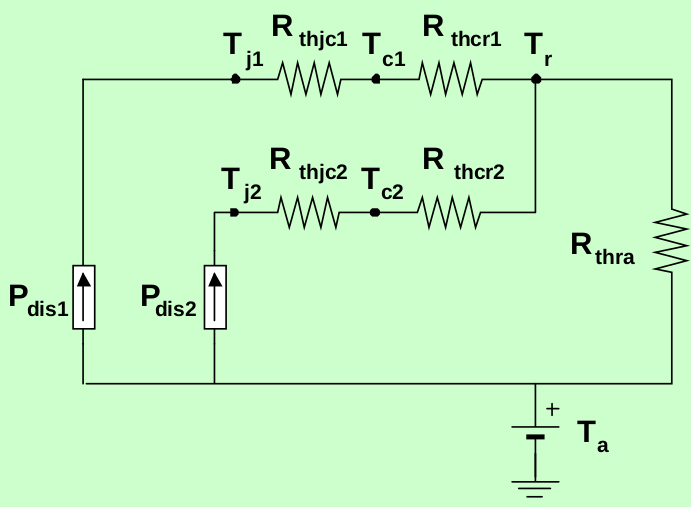
\includegraphics[height=0.4\textwidth]{img/calculo_disipador}
    \caption{Modelo termico estacionario.}
    \label{fig:disipadores}
\end{figure}

En el peor caso, los transistores de potencia 2SC3281 de la etapa de salida y su par complementario 2SA1302
disipan cada uno 18 W, ya que los mismos se utilizan en paralelo.

\begin{equation*}
T_r = R_{thra} * (P_{dis1}+P_{dis2}) + T_a
\end{equation*}

\begin{equation*}
T_r = T_{juntura_{N}} - (R_{t_{j-case}}+R_{t_{c-heat}})*P_{disN}
\end{equation*}

\begin{equation*}
T_r = 130°C - (0.85 °C/W + 0.1 °C/W)*(18*2 W) = 95.8 °C
\end{equation*}

\begin{equation*}
95.8°C = R_{thra}*(18*2*2 W) + 40°C
\end{equation*}

\begin{equation*}
R_{tha} = 0.77 °C/W
\end{equation*}

En la  parte interna de la etapa de salida, tenemos que en el peor caso se disipan 3.25  W por cada transistor.
Haciendo las mismas cuentas con otros valores.


\begin{equation*}
T_r = 120°C - (6.25°C/W + 0.1°C/W)*(3.25W) = 99.36 °C
\end{equation*}

\begin{equation*}
R_{tha} = 9.13 °C/W
\end{equation*}

\paragraph{Disipadores elegidos:}

Para la parte externa de la salida ZD-23 0.65°C/W , elegimos este modelo porque nos da un poco de margen.

\begin{figure}[H]
    \centering
    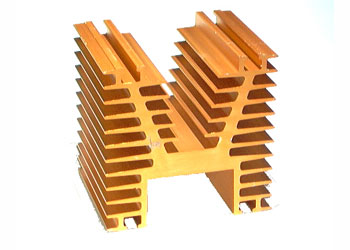
\includegraphics[height=0.4\textwidth]{img/zd23.jpg}
    \caption{Disipador ZD-23}
    \label{fig:diszd23}
\end{figure}


Para parte interna ZD-14 2°C/W, si bien solo necesitamos 9°C/W , elegimos este modelo porque nos da mas margen:

\begin{figure}[H]
    \centering
    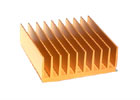
\includegraphics[height=0.4\textwidth]{img/zd14.jpg}
    \caption{Disipador ZD-14}
    \label{fig:diszd14}
\end{figure}